\documentclass{beamer}
\setbeamertemplate{navigation symbols}{}
\usepackage{graphicx,tikz} % Required for inserting images
\usetikzlibrary{calc}
\definecolor{crimson}{RGB}{ 170, 4, 36 }
\definecolor{darkblue}{RGB}{ 4, 47, 170 }
\definecolor{brown}{RGB}{ 111, 71, 2 }
\definecolor{periwinkle}{RGB}{ 90, 177, 204 }
\definecolor{ducksgreen}{HTML}{007030}

\begin{document}

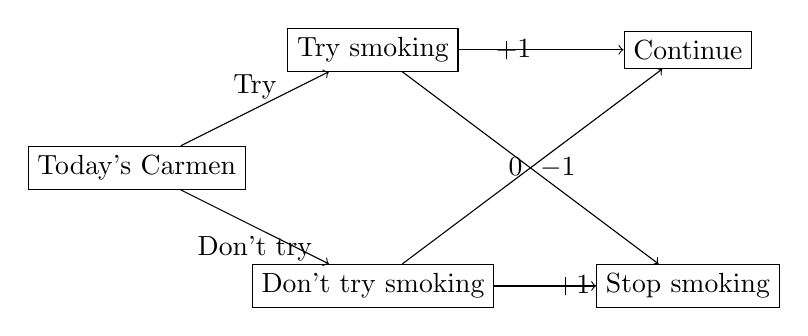
\begin{tikzpicture}[node distance=2cm]
  \node (Carmen) at (-3,0) [draw, 
rectangle] {Today's Carmen};
  
  \node (Try) at (0,1.5) [draw, rectangle] 
{Try smoking};
  \node (Not) at (0,-1.5) [draw, 
rectangle] {Don't try smoking};
  
  \node (Continue) at (4,1.5) [draw, 
rectangle] {Continue};
  \node (Stop) at (4,-1.5) [draw, 
rectangle] {Stop smoking};
  
  \draw[->] (Carmen) -- node [above] {Try} 
(Try);
  \draw[->] (Carmen) -- node [below] 
{Don't try} (Not);
  
  \draw[->] (Try) -- node [left] {$+1$} 
(Continue);
  \draw[->] (Try) -- node [right] {$-1$} 
(Stop);
  
  \draw[->] (Not) -- node [left] {$0$} 
(Continue);
  \draw[->] (Not) -- node [right] {$+1$} 
(Stop);
\end{tikzpicture}

\end{document}
